\documentclass[12pt,xcolor=table,aspectratio=169]{beamer}
\usetheme{Frankfurt}
\usecolortheme{rose}
\usepackage{amsthm}
\usepackage{amsmath}
\usepackage{bbm}
\usepackage{amsfonts}
\usepackage{amssymb}
\usepackage{graphicx}
\usepackage{hyperref}
\usepackage[flushleft]{threeparttable}
\usepackage{tabularx}
\usepackage{booktabs}
\usepackage{siunitx}
\usepackage{tikz}
\usetikzlibrary{decorations.pathreplacing,angles,quotes}
\usepackage{ulem}
%\usepackage{enumitem}% http://ctan.org/pkg/enumitem

%set up course and number

\newcommand{\ClassName}{TBD}
\newcommand{\ClassNumber}{TBD}
\newcommand{\Topic}{TBD}

% Some optional colors. Change or add as you see fit.
%---------------------------------------------------
 \definecolor{ualbertagreen}{HTML}{007C41}
\definecolor{ualbertagold}{HTML}{FFDB05}

\definecolor{calloutgrey}{HTML}{D9D9D9}


%set fonts
\setbeamerfont{subtitle}{size=\large,shape=\scshape,series=\bfseries}
\setbeamerfont{title}{size=\Large,shape=\scshape,series=\bfseries}
\setbeamerfont{author}{size=\large}
\setbeamerfont{date}{size=\large}
\setbeamerfont{caption}{size=\scriptsize}


% Some optional color adjustments to Beamer. Change as you see fit.
%------------------------------------------------------------------
\setbeamercolor{frametitle}{fg=ualbertagreen,bg=white}
\setbeamercolor{title}{fg=ualbertagreen,bg=white}
\setbeamercolor{author}{fg=ualbertagreen,bg=white}
\setbeamercolor{date}{fg=ualbertagreen,bg=white}
\setbeamercolor{local structure}{fg=ualbertagreen}
\setbeamercolor{section in toc}{fg=ualbertagreen,bg=white}
% \setbeamercolor{subsection in toc}{fg=ualbertagreen,bg=white}
\setbeamercolor{footline}{fg=ualbertagreen!50, bg=white}

% definition boxes
\setbeamercolor{block title}{bg=ualbertagreen,fg=white}
\setbeamercolor{block body}{parent=normal text,use=block title,bg=calloutgrey}
%\setbeamercolor{block body}{parent=normal text,use=block title,bg=block title.bg!30!bg}


\setbeamercolor{upper separation line head}{bg=ualbertagreen}
\setbeamercolor{lower separation line head}{bg=ualbertagold}
\setbeamercolor{middle separation line head}{bg=ualbertagold}
\setbeamercolor{frametitle}{fg=ualbertagreen,bg=white}



\setbeamercolor{section in head/foot}{bg=white,fg=ualbertagreen}
\setbeamercolor{author in head/foot}{bg=white,fg=ualbertagreen}
\setbeamercolor{date in head/foot}{bg=white,,fg=ualbertagreen}
\setbeamercolor{title in head/foot}{bg=white,fg=ualbertagreen}

\setbeamercolor{headline}{bg=white,fg=ualbertagreen}




\setbeamercolor*{middle separation line head}{bg=ualbertagreen}
\setbeamercolor*{alerted text}{fg=ualbertagreen}
\setbeamercolor*{example text}{fg=black}
\setbeamercolor*{structure}{fg=black}


\let\Tiny=\tiny



\logo{
   %\ifnum\insertpagenumber>1
   \tikz [remember picture,overlay]
    \node[yshift=.3cm,xshift=1.5cm] at (current page.south west)
        %or: (current page.center)
        {
\includegraphics[width=1in]{../images/UA-ASB-COLOUR.png}};
    %\fi
%
\includegraphics[height=0.8cm]{../images/UA-ASB-COLOUR.png}\vspace{220pt}
}


\setbeamertemplate{title page}{%
  \vbox{}
    \vspace{.5cm}% NEW
  \begingroup
    \centering
    \begin{beamercolorbox}[sep=8pt,center]{title}
      \usebeamerfont{title}\ClassNumber: \ClassName\par%
      \usebeamerfont{title}\inserttitle\par%
     \ifx\insertsubtitle\@empty%
      \else%
        \vskip0.05em%
        {\usebeamerfont{subtitle}\usebeamercolor[fg]{subtitle}\insertsubtitle\par}%
      \fi%
    \end{beamercolorbox}%
    \begin{beamercolorbox}[sep=8pt,center]{author}
      \usebeamerfont{author}\insertauthor
    \end{beamercolorbox}
    \begin{beamercolorbox}[sep=8pt,center]{institute}
      \usebeamerfont{institute}\insertinstitute
    \end{beamercolorbox}

    \vspace{0.5cm}% NEW
    \begin{beamercolorbox}[sep=8pt,center]{date}
      \usebeamerfont{date}\insertdate
    \end{beamercolorbox}\vskip0.05em

      \endgroup
  %\vfill
}


\setbeamertemplate{frametitle}{%
    \insertframetitle\par\vskip-10pt
}



\renewcommand{\ClassName}{Business Economics, Organization and Management}
\renewcommand{\ClassNumber}{BUEC 311}

\setbeamertemplate{headline}{%
\leavevmode%
 \hbox{%
    \begin{beamercolorbox}[wd=\paperwidth,ht=5ex,dp=0ex]{white}%
    \usebeamerfont{headline}\hskip6pt\ClassNumber: \inserttitle\par%
    \insertsectionnavigationhorizontal{\paperwidth}{}{\hskip0pt plus1filll}
    \end{beamercolorbox}%
  }
}

\defbeamertemplate*{footline}{my footline}{%
    \ifnum\insertpagenumber=1
        \Tiny{%
            \hfill%
		\vspace*{1pt}%
            %\insertframenumber/\inserttotalframenumber \hspace*{0.1cm}%
            \newline%
            \color{ualbertagold}{\rule{\paperwidth}{0.4mm}}\newline%
            \color{ualbertagold}{\rule{\paperwidth}{.4mm}}%
        }
  \else%
        \Tiny{%
            \hspace{.66\paperwidth}
            %\vspace{25pt}
            \insertframenumber/\inserttotalframenumber
            \newline%
            \color{ualbertagold}{\rule{\paperwidth}{0.4mm}}\newline%
            \color{ualbertagold}{\rule{\paperwidth}{.4mm}}%
        }%
    \fi%
}


\newenvironment{itemize*}%
  {\begin{itemize}%
    \setlength{\itemsep}{0pt}%
    \setlength{\parskip}{0pt}}%
  {\end{itemize}}


\title{Strategic Behaviour Part I\\
	Game Theory and Business Strategy
}

\date{Fall 2021}

\begin{document}

\section{Overview}


\frame{
	\titlepage
}

\frame{
	\frametitle{Outline}
	\begin{enumerate}
	\item Oligopoly Games
	\item []
     \item Auctions
	\end{enumerate}
}

\frame{
	\frametitle{Strategic Interaction}
	\begin{itemize}
	\item Thus far: We have primarily focused on cases where firms are not interacting strategically.
		\begin{itemize}
		\item But we often need to understand the potential decisions of rivals.
		\item We need a toolbox for understanding strategic decision making.
		\end{itemize}
	\item[]
	\item \underline{Game Theory}: A set of tools used to analyze strategic decision making.
		\begin{itemize}
		\item Idea: Model strategic interactions as a \underline{game} in which \underline{players} interact according to a set of rules.
			\begin{itemize}
			\item Players decide \underline{strategies} based on \underline{payoffs}, the level of \underline{information}, and their \underline{rationality}.
			\item Outcome of a game is a \underline{Nash Equilibrium}; depends on information and rationality.
			\end{itemize}
		\item Game theory can be used to understand strategic behaviour by firms, outcomes in bargaining, and auctions.
		\end{itemize}
	\end{itemize}
}

\frame{
	\frametitle{Outline}
	\begin{enumerate}
	\item \alert{Oligopoly Games}
	\item[]
	\item Auctions
	\end{enumerate}
}

\section{Oligopoly Games}


\frame{
	\frametitle{Oligopoly Games}
	\begin{itemize}
	\item Ex. A duopoly game between American Airlines and United Airlines
		\begin{itemize}
		\item Players and rules:
			\begin{itemize}
			\item \underline{Two players}: American and United, play a \underline{static game} to decide how many passengers to fly per quarter. Each airline's objective is to maximize profit.
			\item \underline{Rules}: Firms announce output levels \underline{simultaneously}, but cannot communicate otherwise (no side deals or coordination is allowed).
			\item \underline{Complete information}: Firms know all strategies and payoffs.
			\end{itemize}
		\item[]
		\item Strategies:
			\begin{itemize}
			\item Each firm's \underline{strategy} is to take one of two available actions: ether choose low output (48k passengers per quarter) or high output (64k passengers per quarter).
			\item Both firms know all strategies and the corresponding payoffs for each firm.
			\item We can summarize these strategies in a payoff matrix (or profit matrix).
			\end{itemize}
		\end{itemize}
	\end{itemize}
}

\frame{
	\frametitle{Oligopoly Games}
	\begin{figure}
	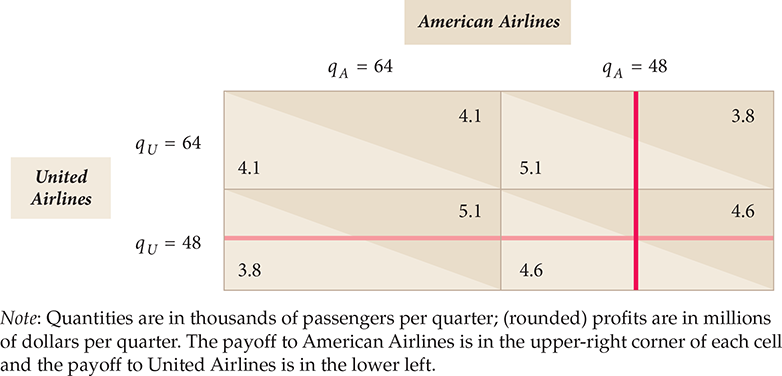
\includegraphics[scale=0.4]{../images/game_theory/au1.png}
	\caption{The Payoffs for American and United}
	\end{figure}
}

\frame{
	\frametitle{Dominant Strategies}
	\begin{itemize}
	\item If one is available, a rational player always uses a \underline{dominant strategy}.
	\end{itemize}
	\begin{definition}[Dominant Strategy]
	A dominant strategy is a strategy that produces a higher payoff (profit) than any other strategy the player can use, no matter what its rivals do.
	\end{definition}
	\begin{itemize}
	\item In our airline duopoly example, high-output (64k) is the dominant strategy for both firms.	
		\begin{itemize}
		\item High output yields the highest profit \textit{regardless of what the other firm is doing}.
		\item Hence, the \underline{dominant strategy solution} is $q_{U} = q_{A} =64$.
		\end{itemize}
	\end{itemize}
}

\frame{
	\frametitle{Payoffs}
	\begin{itemize}
	\item A dominant strategy solution does not necessarily lead to the best outcome for firms.
		\begin{itemize}
		\item In our example, United and American choose strategies that do not maximize their joint or combined profit.
			\begin{itemize}
			\item Each firm could earn \$4.6 million if they both chose to produce a low level of output (48k).
			\end{itemize}
		\item[]
		\item Game between United and American is an example of a \underline{Prisoner's Dilemma}.
			\begin{itemize}
			\item All players have dominant strategies that lead to a profit that is inferior to what they could have achieved if they cooperated.
			\item Individual incentives cause players to choose strategies that do not maximize joint profits.
			\end{itemize}
		\end{itemize}
	\end{itemize}
}

\frame{
	\frametitle{Prisoner's Dilemma Example}
	\begin{itemize}
	\item Suppose that United and American are now choosing whether or not to invest in new planes. Currently, each airline earns a profit of \$25 billion using their old fleet of planes. If American upgrades to new planes and United does not, then American steals some of United's customers and increases its profits to \$35 billion, while United's profits fall to \$10 billion. Similarly, if United upgrades and American does not, United's profits increase to \$35 billion and American's profits fall to \$10 billion. If both airlines upgrade to new planes, then they each will earn \$20 billion. What will each firm do? What will they earn in equilibrium?
	\end{itemize}
}

\frame{
	\frametitle{Best Responses}
	\begin{itemize}
	\item Many games do not have a dominant strategy solution. In this case, we can use the approach of \underline{best response} to determine the outcome of a game.
	\end{itemize}
	\begin{definition}[Best Response]
	A best response is the strategy that maximizes a players payoff (profit) given its beliefs about the strategies of its rivals.
	\end{definition}
	\begin{itemize}
	\item A dominant strategy is a strategy that is a best response to all possible strategies a rival might use.
	\item[]
	\item In the absence of a dominant strategy, each firm can determine its best response to \underline{any possible} strategy chosen by its rivals.
	\end{itemize}
}

\frame{
	\frametitle{Nash Equilibrium}
	\begin{itemize}
	\item Best responses are the basis of a \underline{Nash Equilibrium}.
	\end{itemize}
	\begin{definition}[Nash Equilibrium]
	A Nash equilibrium is a set of strategies such that if, when all other players use these strategies, no player can obtain a higher profit by choosing a different strategy.
	\end{definition}
	\begin{itemize}
	\item In a Nash equilibrium, players are ``best-responding'' to each other.
		\begin{itemize}
		\item This means the Nash equilibrium is self enforcing.
		\end{itemize}
	\item[]
	\item Two steps to find the Nash Equilibrium:
		\begin{enumerate}
		\item Determine each player's best response to any given strategy of the other player.
		\item Check whether pairs of strategies are best responses for both firms; these pairs are Nash equilibria.
		\end{enumerate}
	\end{itemize}
}

\frame{
	\frametitle{Oligopoly Games}
	\begin{itemize}
	\item As an example, consider a more complicated game between American and United.
		\begin{itemize}
		\item Now both firms have 3 possible strategies:
			\begin{enumerate}
			\item High output (96k passengers/quarter).
			\item Medium output (64k passengers/quarter).
			\item Low output (8k passengers/quarter).
			\end{enumerate}
		\item Otherwise, the rules are the same as before:
			\begin{itemize}
			\item Static simultaneous move game.
			\item Perfect information.
			\end{itemize}
		\end{itemize}
	\end{itemize}
}

\frame{
	\frametitle{Oligopoly Games}
	\begin{figure}
	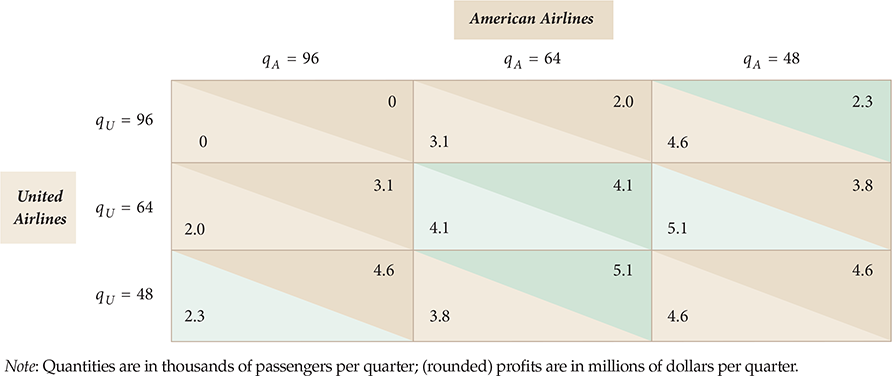
\includegraphics[scale=0.4]{../images/game_theory/au2.png}
	\end{figure}
}

\frame{
	\frametitle{Oligopoly Games}
	\begin{itemize}
	\item Determine equilibrium via two step method:
		\begin{enumerate}
		\item Determine best responses for United:
			\begin{itemize}
			\item If United chooses $q_U=96$, American's best response is $q_{A}=48$.
			\item If United chooses $q_U=64$, American's best response is $q_{A}=64$.
			\item If United chooses $q_U=48$, American's best response is $q_{A}=64$.
			\end{itemize}
		\item[] And for American:
			\begin{itemize}
			\item If American chooses $q_A=96$, United best response is $q_{U}=48$.
			\item If American chooses $q_A=64$, United best response is $q_{U}=64$.
			\item If American chooses $q_A=48$, United best response is $q_{U}=64$.
			\end{itemize}
		\item[]
		\item Determine the Nash Equilibrium
			\begin{itemize}
			\item The Nash equilibrium is $q_{A} = q_{U} = 64$.
			\item This outcome is a Nash equilibrium because neither firm wants to deviate from its strategy \textit{given what the other firm is doing.}
			\item Note: The Nash Equilibrium does not maximize joint profits.
			\end{itemize}
		\end{enumerate}
	\end{itemize}
}

\frame{
	\frametitle{Oligopoly Games}
	\begin{itemize}
	\item In general, whether or not the Nash equilibrium maximizes the combined payoff to players (i.e. profits for firms) depends on the payoff matrix.
	\item[]
	\item As an example, consider a static game where firms decide to `advertise' or `not advertise'.
	\item[]
	\item The effects of advertising depend on whether advertising brings new customers into the market.
	\end{itemize}
}

\frame{
	\frametitle{Oligopoly Games}
	\begin{figure}
	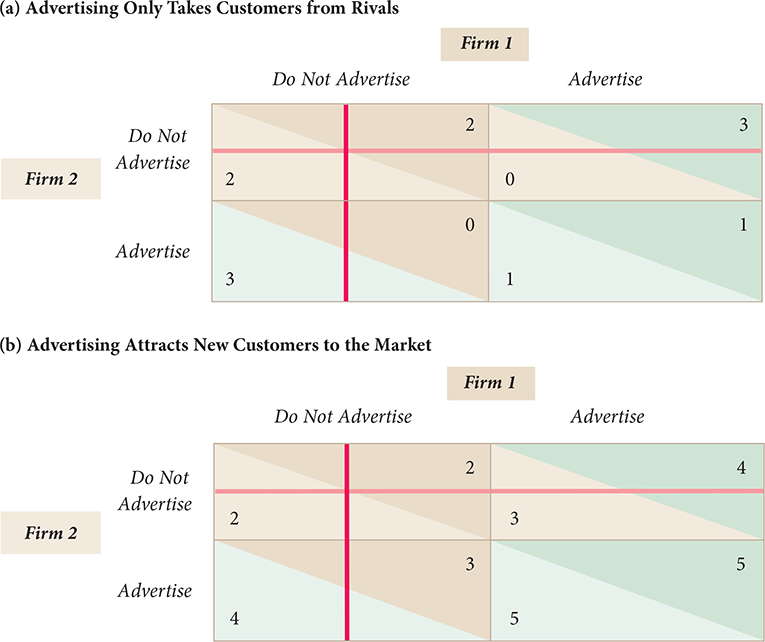
\includegraphics[scale=0.3]{../images/game_theory/advertising.png}
	\end{figure}
}

\frame{
	\frametitle{Oligopoly Games}
	\begin{itemize}
	\item Example highlights a phenomenon often observed in practice:
		\begin{itemize}
		\item In oligopolistic markets, the effect of firm advertising depends on whether it helps (increases the size of the overall market) or hurts (steals customers) rivals.
		\end{itemize}
	\item[]
	\item In some industries, advertising primarily steals customers from rivals.
		\begin{itemize}
		\item E.g. market for cola; market for erectile dysfunction drugs.
		\end{itemize}
	\item[]
	\item In other industries, advertising by any firm increases the size of the market.
		\begin{itemize}
		\item E.g. market for beer; market for cigarettes.
		\end{itemize}
	\item[]
	\item It is possible to observe market size and business stealing effects simultaneously.
		\begin{itemize}
		\item E.g. Fast food; CPUs.
		\end{itemize}
	\end{itemize}
}

\section{Auctions}

\frame{
	\frametitle{Outline}
	\begin{enumerate}
	\item Oligopoly Games
	\item[]
	\item \alert{Auctions}
	\end{enumerate}
}


\frame{
	\frametitle{Auctions}
	\begin{definition}[Auction]
	A sale in which a good or service is sold to the highest bidder.
	\end{definition}
	\begin{itemize}
	\item Game theory can be used to understand behaviour in auctions.
		\begin{itemize}
		\item An auction is a game in which players (called \underline{bidders}) devise bidding strategies without knowing the payoff functions of other players.
		\item Bidders need to know the rules of the game:
			\begin{itemize}
			\item The number of units being sold.
			\item The format of bidding.
			\item The value that potential bidders place on the good.
			\end{itemize}
		\end{itemize}
	\end{itemize}
}

\frame{
	\frametitle{Auctions}
	\begin{itemize}
	\item Auctions are frequently used in practice:
		\begin{itemize}
		\item Government auctions:
			\begin{itemize}
			\item Government procurement, auctions for electricity and transport markets, auctions to concede portions of the airwaves for radio stations, mobile phones and wireless internet access; auctions for oil and gas leases.
			\end{itemize}
		\item[]
		\item Market transactions:
			\begin{itemize}
			\item Goods commonly sold at auction are natural resource such as timber and drilling rights for oil, as well as houses, cars, agricultural products, horses, antiques and art. And of course, goods online in sites like eBay.
			\end{itemize}
		\end{itemize}
	\end{itemize}
}

\frame{
	\frametitle{Elements of Auctions}
	\begin{itemize}
		\item Number of units: auctions can be used to sell one or many units of a good.
		\item Format of bidding:
			\begin{itemize}
			\item  \underline{English auction}: Ascending-bid auction process where the good is sold to the last bidder for the highest bid. Commonly used to sell art/antiques.
			\item \underline{Dutch auction}: Descending-bid auction process where the seller reduces the price until someone accepts it and buys at that price. Often used in government procurement.
			\item \underline{Sealed-bid auction}: Bidders submit bids simultaneously without seeing anyone else's bid and highest bidder wins. In a 1st price sealed-bid auction, the winner pays its own, highest bid. In a 2nd price sealed-bid auction, the winner pays the amount bid by the 2nd highest bidder.
			\end{itemize}
		\item Value:
			\begin{itemize}
			\item \underline{Private value}: Individual bidders know how much the good is worth to them, but not how much other bidders value it.
			\item \underline{Common value}: The good has the same value to everyone, but no bidder knows exactly what that value is.
			\end{itemize}
		\end{itemize}
}

\frame{
	\frametitle{Second Price Sealed Bid Auctions}
	\begin{itemize}
	\item Rules:
		\begin{itemize}
		\item Each bidder has a different private value for a single indivisible good.
		\item Bidders simultaneously submit sealed bids without knowledge of other bids.
		\end{itemize}
	\item Design of auction means that amount that you bid affects whether you win, but it does not affect how much you pay if you win (which is equal to the second-highest bid).
	\item Best strategy: Bid your highest value.
		\begin{itemize}
		\item This strategy weakly dominates all others.
		\item Ex: Suppose that you value a folk art carving at \$100. If you bid \$100 and win, your $CS=100 - \text{2nd price}$. If you bid less than \$100, you risk not winning. If you bid more than \$100, you risk ending up with negative $CS$.
		\item Thus, bidding \$100 leaves you \textit{at least as well off} as bidding any other value.
		\end{itemize}
	\end{itemize}
}

\frame{
	\frametitle{English Auctions}
	\begin{itemize}
	\item Rules:
		\begin{itemize}
		\item Each bidder has a different private value for a single indivisible good.
		\item Ascending-bid auction process where the good is sold to the last bidder for the highest bid.
		\end{itemize}
	\item Design of auction means that amount you bid affects whether you win and how much you pay.
	\item Best strategy: Raise the current highest bid as long as that value is less than the value you place on the good.
		\begin{itemize}
		\item Ex: Again suppose that you value a folk art carving at \$100. If you bid an amount $b$ and win, $CS =100- b$. $CS$ is positive or zero for $b\leq100$, but negative if $b>100$. So it is best to raise bids up to \$100 and stop there.
		\item If all participants bid up to their value, the winner will pay slightly more than the value of the second-highest bidder. Thus, the outcome of an English auction is essentially the same is a in a sealed-bid, second-price auction.
		\end{itemize}
	\end{itemize}
}

\frame{
	\frametitle{Other Auctions}
	\begin{itemize}
	\item Two other common private value auctions:
		\begin{itemize}
		\item Dutch Auction: Descending-bid auction where the seller reduces the price until someone accepts the offered price and buys at that price.
		\item First-Price Sealed-Bid Auction: Bidders submit bids simultaneously without seeing other bids. Highest bidder wins and pays amount of bid.
		\end{itemize}
	\item In both cases, the amount that you bid affects whether you win and pay.
	\item The best strategy in both auctions is to bid an amount that is equal to, or slightly greater than what you expect will be the second-highest bid, given that your value is the highest.
		\begin{itemize}
		\item Bidders shade bids to less than their value to balance the effect of decreasing the probability of winning and increasing $CS$. Bid depends on beliefs about strategies of rivals.
		\end{itemize}
	\end{itemize}
}

\frame{
	\frametitle{Auctions}
	\begin{itemize}
	\item Key point: Expected outcome is the same across private value auctions.
		\begin{itemize}
		\item Winner is the person with the highest value, and the winner pays roughly the second-highest value.
		\end{itemize}
	\item[]
	\item Is there any reason that a seller still might choose one format over an alternative?
	\end{itemize}
}

\frame{
	\frametitle{Auctions}
	\begin{itemize}
	\item Key feature of \underline{common-value} auctions: the Winner's Curse.
		\begin{itemize}
		\item Winner's bid exceeds the value of item up for bid; winner pays too much.
		\item Occurs due to uncertainty about the true value of the good.
			\begin{itemize}
			\item E.g. Timber land auctions/auctions for oil and gas leases.
			\end{itemize}
		\end{itemize}
	\item Best strategy to avoid Winner's Curse: Shade/reduce bids to below estimates of value.
		\begin{itemize}
		\item The amount of reduction depends on number of other bidders; more bidders $\implies$ more likely winning bid is an overestimate.
		\end{itemize}
	\item While Winner's Curse is a well known phenomenon, there is strong empirical evidence it continues to happen in practice (e.g in the corporate acquisition market).
		\begin{itemize}
		\item One possible explanation: Bounded rationality.
		\end{itemize}
	\end{itemize}
}

\frame{
	\frametitle{Takeaways}
	\begin{enumerate}
	\item Insights from game theory can be used to improve outcomes when making strategic decisions.
	\item[]
	\item Bargaining can lead to efficient outcomes.
	\item[]
	\item Best strategy in most auctions is to bid your valuation, but it may be useful to shade bids to avoid the Winner's Curse.
	\end{enumerate}
}

\end{document}

